\documentclass[aps,pra,notitlepage,amsmath,amssymb,letterpaper,12pt]{revtex4-1}
\usepackage{amsthm}
\usepackage{graphicx}
%  Above uses the Americal Physical Society template for Physical Review A
%  as a reasonable and fully-featured default template
 
%  Below define helpful commands to set up problem environments easily
\newenvironment{definition}[2][Definition]{\begin{trivlist}
\item[\hskip \labelsep {\bfseries #1}\hskip \labelsep {\bfseries #2.}]}{\end{trivlist}}
\newenvironment{solution}{\begin{proof}[Solution]}{\end{proof}}
 
% --------------------------------------------------------------
%                   Document Begins Here
% --------------------------------------------------------------
 
\begin{document}
 
\title{Calculus}
\author{Atabak Pouya}
\affiliation{CS 510, Schmid College of Science and Technology, Chapman University}
\date{\today}

\maketitle

\section{Derivative} % Specify main sections this way

% x.yz is the problem number
\begin{definition}{1.1}
The derivative of $f(x)$ with respect to $x$ is $f'(x)$ and defined as :
\end{definition}
 
\begin{proof} %You can also use proof in place of solution
 derivative is the slope of a line at a specific point
\begin{align}
f'(x) = \lim_{x \rightarrow 0} \frac{f(x+\Delta{x})-f(x)}{\Delta{x}}
\end{align}
In this equation, we are saying
find the slope of the tangent line between two points when you add almost zero to go from the first x value to the next.
% Use align environments for equations. The \\ is a newline character. The & is the alignment character.
% Using align* or \nonumber on each line removes equation numbers
\end{proof}



FIG. 1 illustrates the (1) on a curve.

\begin{figure}[h!] % h forces the figure to be placed here, in the text
  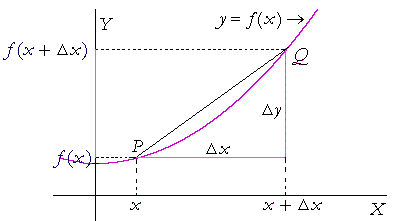
\includegraphics[width=0.4\textwidth]{Secant.png}  % if pdflatex is used, jpg, pdf, and png are permitted
  \caption{Secant of line P.}
  \label{fig:figlabel}
\end{figure}

Since $\Delta{x}$ is the variable that approaches 0, $x$ remains constant, and that limit will be a function of x.  Since it will be derived from $f(x)$, we call it the derived function or the derivative of $f(x)$
 
% Repeat as needed
 
\end{document}
